\chapter{Results\markboth{Results}{}}

This section provides a detailed report of the results obtained from the trained model. It presents the outcomes of various tests and performance metrics without engaging in evaluation or discussion. The purpose of this section is to systematically document the model's results, setting the foundation for deeper analysis in subsequent sections.

\section{Model's Performance}
The following sections offer a comprehensive report on the performance of the trained model. This includes results from multiple assessment methods and performance metrics. Key visualizations, such as the Calibration Curve, which illustrates the relationship between predicted probabilities and actual outcomes, and the Confusion Matrix, which details the model's classification accuracy across all classes, are presented. These results provide a clear and organized summary of the model's performance, which will be further evaluated and discussed in later sections.
\subsection{Calibration Curve}

The calibration curve provides insights into how well the model's predicted probabilities align with the actual outcomes. This analysis is crucial for understanding whether the model's confidence in its predictions is justified.

\begin{figure}[H]
\centering
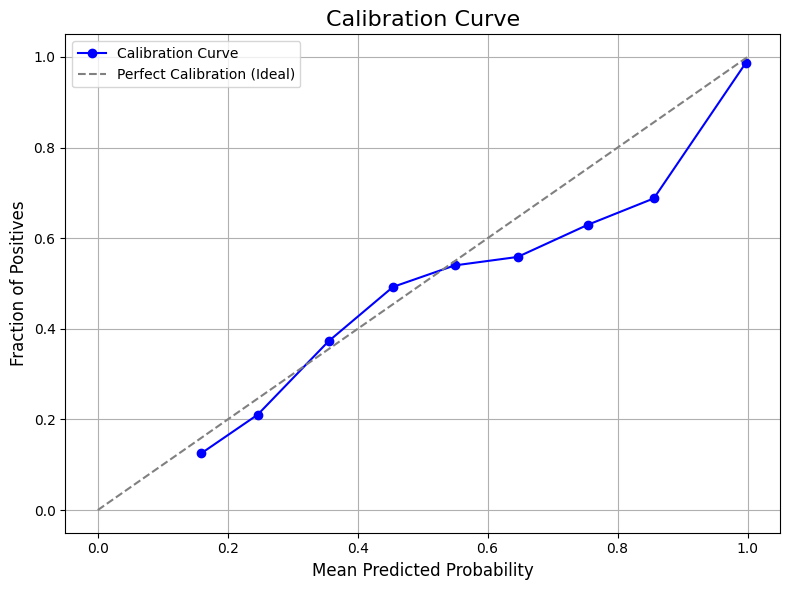
\includegraphics[width=0.8\textwidth]{images/figure15.png}
\caption{Calibration Curve showing the relationship between predicted probabilities and the fraction of positives.}
\label{fig:calibration_curve}
\end{figure}

\subsubsection{Below the Diagonal (Underconfidence)}
For lower predicted probabilities (approximately 0.1 to 0.4), the calibration curve lies \textbf{below} the ideal diagonal line. This behavior indicates that the model is \textbf{underconfident} in its predictions, predicting lower probabilities than the actual observed outcomes.

\subsubsection{Near the Diagonal (Well-Calibrated)}
In the mid-range probabilities (around 0.5 to 0.7), the curve aligns closely with the ideal line. This suggests that the model's predictions in this range are \textbf{well-calibrated}, with predicted probabilities accurately reflecting the true outcomes.

\subsubsection{Above the Diagonal (Overconfidence)}
For higher predicted probabilities (approximately 0.8 to 0.9), the curve rises \textbf{above} the diagonal. This indicates that the model becomes \textbf{overconfident}, predicting higher probabilities than what is observed in reality.

\subsubsection{Sharp Rise at 1.0}
At the highest predicted probability (1.0), the curve nearly touches the ideal calibration line. This suggests that predictions made with full confidence are relatively accurate.

\subsection{Confusion Matrix}

The analysis of the confusion matrix reveals comprehensive insights into the model's performance across various classes. The \textbf{overall accuracy} stands at approximately \textbf{95.61\%}, confirming the model's high capability in accurately classifying the input data. This strong performance indicates effective generalization and robustness across the 43 distinct classes.

\begin{figure}[H]
    \centering
    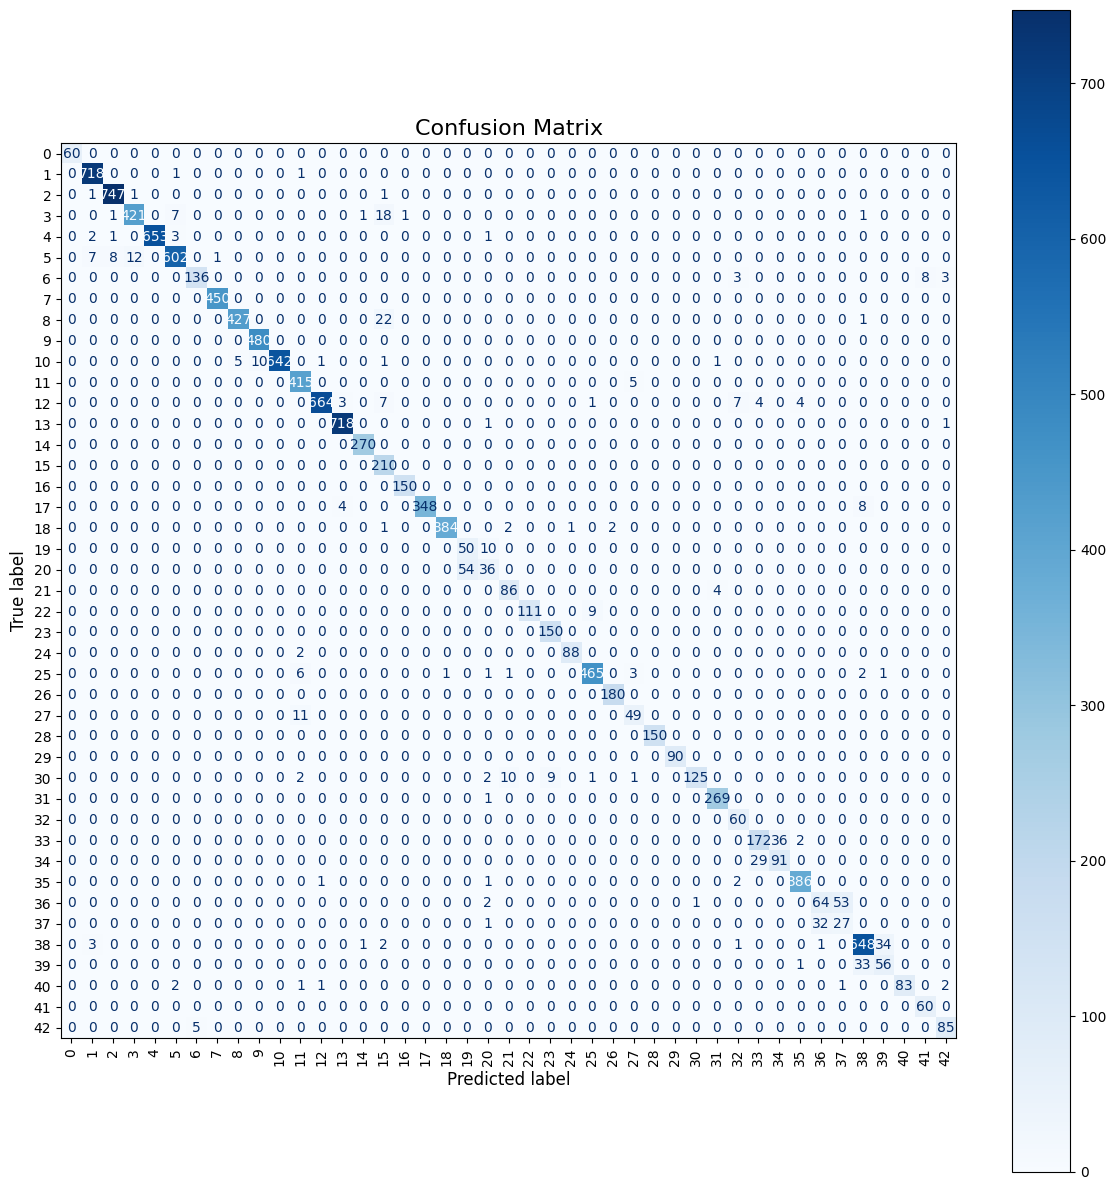
\includegraphics[width=0.8\textwidth]{images/figure13/figure14.png}
    \caption{Confusion Matrix.}
    \label{fig:fig14}
  \end{figure}

Further examination of the model's behavior is reflected in the class-wise metrics. The \textbf{average precision} is \textbf{90.69\%}, indicating that when the model makes a positive prediction for a class, it is correct over 90\% of the time. The \textbf{average recall} is slightly higher at \textbf{91.36\%}, meaning the model successfully identifies more than 91\% of actual instances for each class. This balance between precision and recall results in an \textbf{average F1-score} of \textbf{90.72\%}, highlighting the model's consistent performance across various categories.

The confusion matrix also highlights misclassification trends. While the majority of predictions align with true labels, some off-diagonal elements reveal instances where certain classes are confused. These misclassifications could result from visual similarities between specific classes or limited training samples for those categories.

\section{Tests}
The following table summarizes the accuracy results of the model in both standalone and VANET simulation modes across different test conditions:

\begin{table}[h!]
    \centering
    \begin{adjustbox}{width=\textwidth}
    \begin{tabular}{|l|c|c|c|}
        \hline
        \textbf{Condition} & \textbf{Standalone Model Accuracy (\%)} & \textbf{VANET Simulation Accuracy (\%)} & \textbf{Difference (\%)} \\ \hline
        Normal (No Alteration) & 95.68 & 95.68 & 0.00 \\ \hline
        Brightness Adjustment & 95.51 & 95.46 & -0.05 \\ \hline
        Motion Blur & 64.08 & 66.37 & +2.29 \\ \hline
        Rotation & 62.15 & 77.66 & +15.51 \\ \hline
    \end{tabular}
    \end{adjustbox}
    \caption{Accuracy comparison between standalone model and VANET simulation across various conditions.}
    \label{tab:accuracy_comparison}
\end{table}


\begin{itemize}
    \item \textbf{Normal Condition:} Both the standalone model and the VANET simulation achieved an accuracy of 95.68\%. This identical performance is due to the deterministic nature of the model, which produces the same output when given the same input, rendering the consensus mechanism ineffective in this case.
    
    \item \textbf{Brightness Adjustment:} The standalone model achieved 95.51\% accuracy, very close to the original performance. This robustness is attributed to the model being trained on images with varying brightness levels. The VANET simulation achieved 95.46\%, with a negligible difference of 0.05\%, indicating minimal impact due to the model's high baseline performance.
    
    \item \textbf{Motion Blur:} The standalone model's accuracy dropped to 64.08\%. However, the VANET simulation improved the accuracy to 66.37\%, reflecting a modest 2.29\% enhancement due to the consensus mechanism, which helped correct some misclassifications.
    
    \item \textbf{Rotation:} This condition showed the most significant improvement. The standalone model achieved 62.15\% accuracy, while the VANET simulation achieved 77.66\%, marking a substantial 15.51\% increase. This improvement highlights the effectiveness of the consensus mechanism in handling more challenging distortions.
\end{itemize}